\documentclass[tikz,border=8pt]{standalone}
\usepackage{amsmath}
\usetikzlibrary{arrows.meta,positioning,fit,calc}

\begin{document}
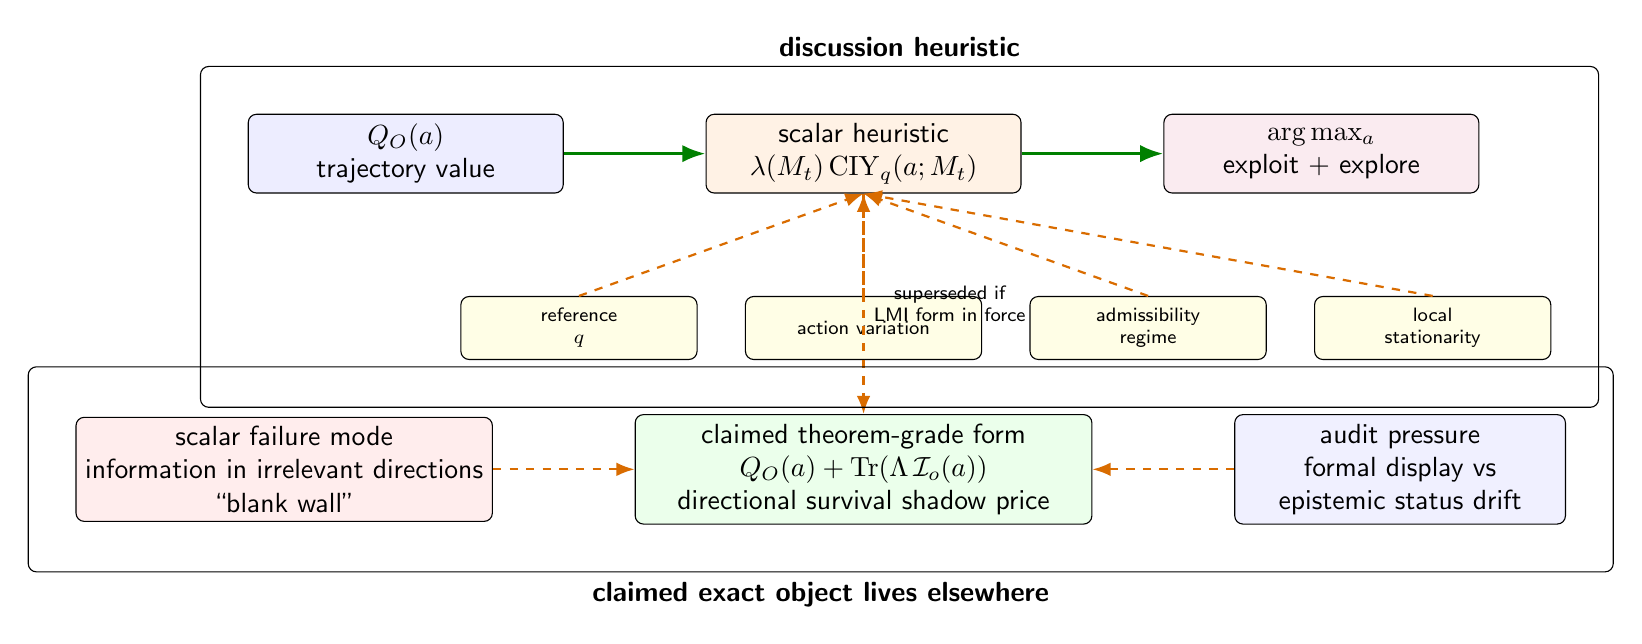
\begin{tikzpicture}[
  font=\sffamily,
  box/.style={draw, rounded corners=3pt, align=center, minimum width=40mm, minimum height=10mm, fill=white},
  small/.style={draw, rounded corners=3pt, align=center, minimum width=30mm, minimum height=8mm, fill=white, font=\sffamily\scriptsize},
  arrow/.style={-Latex, thick, draw=black!65},
  good/.style={-Latex, very thick, draw=green!50!black},
  warn/.style={-Latex, thick, dashed, draw=orange!85!black},
  note/.style={align=center, font=\sffamily\scriptsize}
]

\node[box, fill=blue!7] (value) {$Q_O(a)$\\trajectory value};
\node[box, right=18mm of value, fill=orange!10] (scalar) {scalar heuristic\\$\lambda(M_t)\,\mathrm{CIY}_q(a;M_t)$};
\node[box, right=18mm of scalar, fill=purple!8] (choice) {$\arg\max_a$\\exploit + explore};

\draw[good] (value) -- (scalar);
\draw[good] (scalar) -- (choice);

\node[small, below=13mm of scalar, fill=yellow!10] (gate1) {action variation};
\node[small, right=6mm of gate1, fill=yellow!10] (gate2) {admissibility\\regime};
\node[small, left=6mm of gate1, fill=yellow!10] (gate0) {reference\\$q$};
\node[small, right=6mm of gate2, fill=yellow!10] (gate3) {local\\stationarity};
\foreach \g in {gate0,gate1,gate2,gate3} {
  \draw[warn] (\g.north) -- (scalar.south);
}

\node[box, below=28mm of scalar, fill=green!8, minimum width=58mm] (matrix)
  {claimed theorem-grade form\\$Q_O(a)+\mathrm{Tr}(\Lambda\,\mathcal{I}_o(a))$\\directional survival shadow price};
\draw[warn] (scalar) -- node[right, note] {superseded if\\LMI form in force} (matrix);

\node[box, left=18mm of matrix, fill=red!7, minimum width=42mm] (blank)
  {scalar failure mode\\information in irrelevant directions\\``blank wall''};
\draw[warn] (blank) -- (matrix);

\node[box, right=18mm of matrix, fill=blue!6, minimum width=42mm] (status)
  {audit pressure\\formal display vs\\epistemic status drift};
\draw[warn] (status) -- (matrix);

\node[draw, rounded corners=3pt, fit=(value)(scalar)(choice)(gate0)(gate1)(gate2)(gate3), inner sep=6mm,
  label={[font=\sffamily\bfseries]above:discussion heuristic}] {};
\node[draw, rounded corners=3pt, fit=(blank)(matrix)(status), inner sep=6mm,
  label={[font=\sffamily\bfseries]below:claimed exact object lives elsewhere}] {};

\end{tikzpicture}
\end{document}
